\chapter{An Augmented Quantum Threshold Scheme}
\label{ch3}

As we have shown above, one of the main limitations of QC comes from the no-cloning theorem. The first idea we pose attempts to circumvent this limitation. 

If we already begin with two identical copies of a quantum state, then what does this do, if anything, to change the limitations surrounding the value of $t$ with respect to $n$? What if we have $k$ copies? What schemes are realizable in this new formulation? In this section, we will explore the properties of such a scheme. We will call this an augmented quantum threshold scheme. Let us formalize this idea and explore its consequences below:

\theoremstyle{definition}
\begin{definition}{Augmented Quantum Threshold Scheme.}
     This is a QTS that assumes that we being with $k$ identical copies of a quantum state prepared in advance. As with the normal QTS, we need at least $t$ individuals to come together to recover the secret quantum state. We will denote an augmented QTS as $[t,n,k]$.
\end{definition}

\section{Preliminary thoughts}

Let's consider the case of $k=2$. If we consider just the consequences of the no-cloning theorem, an extension of Theorem \ref{qss-disjoint} can be posed as follows:

\begin{theorem}
    In any valid $((t,n,2))$ scheme, any three authorized subsets cannot be pair-wise disjoint.
\end{theorem}

And a generalization to the case with $k$ identical copies:

\begin{theorem}
    In any valid $((t,n,k))$ scheme, any $k+1$ authorized subsets cannot be pair-wise disjoint.
\end{theorem}

We can also extend Theorem \ref{qts} in a similar manner:

\begin{theorem}
	\label{qts2}
	A QTS $((t,n, 2))$ exists only if $t > \frac{n}{3}$.
\end{theorem}

\begin{theorem}
	\label{qtsk}
	A QTS $((t,n, k))$ exists only if $t > \frac{n}{k+1}$.
\end{theorem}

Each of the proofs of these theorems are almost identical to that of Theorem \ref{qss-disjoint}. However, these theorems only present to us what \textbf{could} be possible. Realizability is a differnet question. It is not immediately obvious that Gottesman's Theorem \ref{monotone-gamma}

The simplest case that is non-trivial is to ask about a $[2,4,2]$ scheme. Using 2 identical copies of a quantum state, is it possible to implement a scheme among 4 individuals such that only 2 or more people need to come together to recover the secret? The answer is yes. We employ a strategy where we superimpose two access structures on top of one another. Let the two copies of our quantum secret be $\ket{\psi_1}, \ket{\psi_2}$, and let the participants be labeled $p_1, p_2, p_3, p_4$. The diagram below shows how we implement the scheme. Each node corresponds to one participant, and the red edges denote authorized subsets of size 2 that are a part of the access structure $\Gamma_1$ of $\ket{\psi_1}$. Blue edges correspond to $\Gamma_2$, which is the access structure of $\ket{\psi_2}$:


\begin{figure}[h]
	\label{fig:2-4-2}
	\begin{center}
		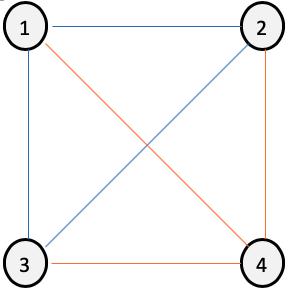
\includegraphics[width=0.5\textwidth]{Images/ch3-fig1.png}
	\end{center}
	\caption{An image of the access structure for a $((2,4,2))$ threshold scheme, using two copies of the quantum secret.}
\end{figure}


The scheme is as follows: $\Gamma_1 = \{p_1p_2,p_2p_3,p_3p_1\}$ and $\Gamma_2 = \{p_1p_4,p_2p_4,p_3p_4\}$. Notice that in each case, we satisfy Theorem \ref{qss-disjoint}.

How can we generalize this strategy? Notice that in the case of the $((2,4,2))$ scheme, we need the union $\Gamma_1 \cup \Gamma_2$ to consist of all subsets of size 2. Each of these access structures must satisfy Theorem \ref{qss-disjoint}. So, in general, a $((t,n,k))$ scheme is realizable if we can take all subsets of size $t$ of the $n$ participants and divide them into $k$ groups, where each group consists of an access structure that satisfies Theorem \ref{qss-disjoint}. 

Let's dive deeper into augmented threshold schemes of the form: $((t,n,2))$. What would be helpful to us is a representation of this problem that allows us to better reason about the authorized subsets contained in the access structures. So, instead of having a formulation like the one above where the vertices are individual participants and the edges are the authorized subsets, let's make each authorized subset a vertex, and use the edges between those vertices to represent some relationship between the authorized subsets.

One option would be to draw an edge between two vertices if they have a non-empty intersection. However, we will opt for the complement of this: we will \textbf{draw an edge between two vertices, representing two authorized subsets, if they are disjoint}. We should give a name to this representation:

\theoremstyle{definition}
\begin{definition}{Access Structure Graph.}
	We define an \textbf{access structure graph} of $\Gamma$ to be the graph $G = (V,E)$, where there is a vertex $v \in V$ for each authorized subset $A \in \Gamma$. The edgeset $E$ contains an edge between each pair of vertices if their corresponding authorized subsets are disjoint.
\end{definition}

Let's show the access structure graph respresentation for Figure 3.1:

\begin{figure}[h]
	\label{2-4-2-label}
	\begin{center}
		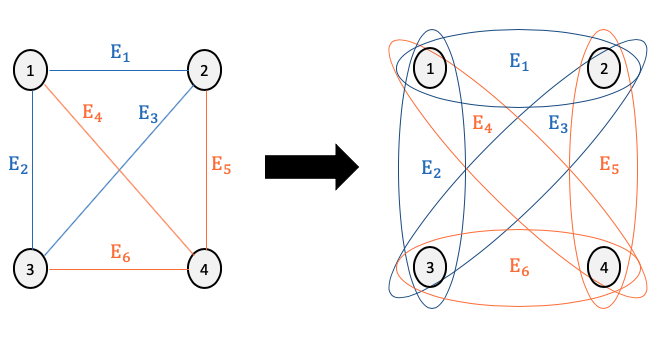
\includegraphics[width=0.8\textwidth]{Images/ch3-fig2.png}
	\end{center}
	\caption{First, we label the edges and show us grouping vertices into their respective authorized subsets. Each edge represents an authorized subset.}
\end{figure}

\begin{figure}[h]
	\label{2-4-2-graph}
	\begin{center}
		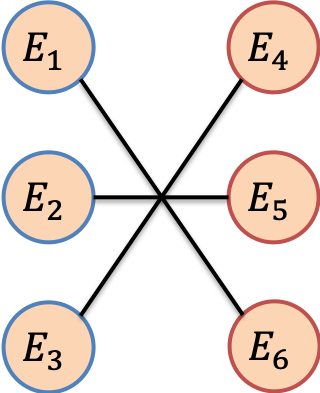
\includegraphics[width=0.3\textwidth]{Images/ch3-fig3.png}
	\end{center}
	\caption{In this figure, we have turned each authorized subset into a vertex, and have drawn an edge between disjoint authorized subsets.}
\end{figure}

\begin{remark}
	Observe that we have actually done two graphical transformations on Figure 3.1. First, we take the Line Graph of Figure 3.1, then we take the complement of that resulting graph. This formulation works best for cases where the authorized susbets are of size 2, but it is interesting to note nontheless.
\end{remark}

The representation illustrated in Figure 3.3 is useful to us because properties of the graph now give reveal properties of the realizability of their corresponding quantum threshold schemes. Before we get to that, let's talk about graph-coloring:

\theoremstyle{definition}
\begin{definition}{Chromatic Color}
	The \textbf{chromatic color} of a graph $\chi(G)$ is the maximum number of colors needed in order to color the vertices of the graph in such a way that vertices of the same color are not adjacent.
\end{definition}

\begin{remark}
	Observe that the chromatic color of the access structure graph of $\Gamma$ must be 2 for $((t,n,2))$- threshold quantum secret sharing schemes.
\end{remark}

What is even better for $((t,n,2))$ schemes is the fact that another name for graphs with $\chi(G)=2$ is \textbf{bipartite}.

\theoremstyle{definition}
\begin{definition}{Bipartite Graph}
	A \textbf{bipartite graph} is one in which the vertices can be separated into two groups. There are no edges between the vertices in any one group.
\end{definition}

A quick look at Figure 3.3 reveals that the graph is indeed bipartite, again verifying that $((2,4,2))$ is a valid scheme. A well-known result in graph theory is as follows:

\begin{theorem}
	\label{bipartite}
	A graph $G$ is bipartite if and only if $G$ does not contain any odd cycles.
\end{theorem}

We can use Theorem \ref{bipartite} to also show that $((3,6,2))$ is also a valid scheme, but that $((2,5,2))$ and $((3,7,2))$ are \textbf{not} valid schemes.


